\chapter{The Friedmann model of the universe}
After spending some time mastering the physical and mathematical tools we need (namely special and general relativity), now we are finally ready for a first approach to the study of modern cosmology; what we will examine in this section is the so called Friedmann model of the universe, which is the simplest model current observations suggest about the cosmos on its largest scales. Observations of the uniformity of the Cosmic Microwave Background (CMB) (see Figure \ref{cmb})and of the redshift of galaxies, already treated in the previous chapter, suggest that, at a first apporximation, our observable universe can be modeled as a uniform expanding ball, filled by some homogeneous fluid that triggers the expansion according to the rules of general relativity. We will be a lot more precise in the following paragraphs.

\begin{figure}
\begin{center}
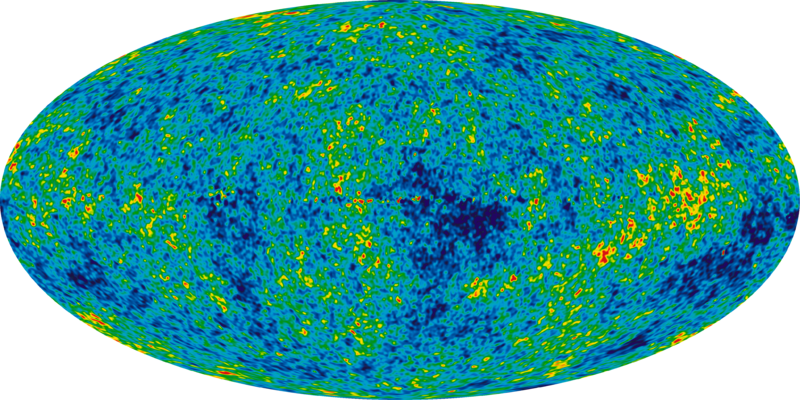
\includegraphics[scale=0.5]{Draw/wmap}
\label{}
\end{center}
\caption{A picture of the temperature Cosmic Microwave Background across the sky, from the experiment WMAP: the fluctuations in temperature from red to blue spots have a relative magnitude $\delta T/T\sim 10^{-5}$.  Credit for the image \url{http://apod.nasa.gov/apod/ap030212.html}}
\label{cmb}
\end{figure}

\section{A uniform ball} 
As stated before, the uniformity of the temperature of the CMB (with fluctuations of relative order $10^{-5}$), measured all across the sky, suggests that our special observation point, Earth, has no special role at all in the universe physical picture: this can be stated as the so called \textit{cosmological principle}, which says that \textit{every observer in the universe} (at rest), will experience the same cosmology, and will get the same results in any observational experiment. This also mean, that all all observers \textit{at rest} (we will explain what this means in the following), will agree on the measurement of time, and we will call this common time reference $t$ ($t=0$ being the beginning of the universe, the Big Bang). In each one of these \textit{at rest} reference frames, we can hence say that our metric will be something like
\begin{equation}
\label{frwsymb}
ds^2=-c^2dt^2+ds_3^2
\end{equation}    
Where $ds_3^2$ is the spacial part of the metric (that involving $dx,dy,dz$) and depends on the spatial geometry of our universe, i.e. on how we measure \textit{spatial} distances. The fact that the universe is homogeneous, as suggested by observations, tells us that $ds_3^2$ cannot be arbitrary, but must satisfy this homogeneity assumption. You can convince yourselves that there are only three possible types of spatial metric that satisfy this requirement, namely a flat metric with curvature $k=0$, a positively curved metric with constant curvature $k=1/R^2$ or a negatively curved metric with constant curvature $k=-1/R^2$. Note that if we want do describe a curved universe, we must specify a curvature scale length, $R$ (the ''radius of curvature'') as pointed out in chapter 2. 
\subsection{The flat case}
If the universe were flat, with no curvature, then the spatial metric would just be the one you are already familiar with in ordinary euclidean space, in which we measure distances with the pythagorean theorem (in coordinates $(x,y,z)$)
\begin{equation}
ds_3^2=dx^2+dy^2+dz^2
\end{equation}
We usually like to use spherical coordinates $(r,\theta,\phi)$, in which the metric becomes that of equation (\ref{metspher})
\begin{equation}
ds_3^2=dr^2+r^2(d\theta^2 + \sin^2{\theta}d\phi^2)
\end{equation}
\subsection{Positive curvature: the sphere case}
If our universe were positively curved, we would model it as a sphere of radius $R$, because this is the only space that has constant positive curvature; the only difference from what we already saw, is that this sphere would be three dimensional (a so called 3-sphere, or $S^3$), not two dimensional as the spheres we saw in chapter 2. How do we model such a sphere? A 3-sphere is a three dimensional subset of a 4 dimensional eucliudean space with coordinates $(x,y,z,w)$; this subset has to satify the constraint
\begin{equation}
x^2+y^2+z^2+w^2=R^2
\end{equation}
Since on this four dimensional space we measure distances with the usual euclidean metric 
\begin{equation}
\label{positive4d}
ds_4^2=dx^2+dy^2+dz^2+dw^2
\end{equation}
If this is how we measure distances on all space,we want to understand on how this four dimensional metric translates into a three dimensional metric on our 3-sphere; this is easily done in spherical coordinates $(r,\theta,\phi)$, which give us a very good parametrization of the sphere (notice that we use only three coordinates because the sphere is a three dimensional subset of this four dimensional space) 
\begin{displaymath}
\left \{ \begin{array}{l}x=r\sin{\theta}\cos{\phi} \\ 
y=r\sin{\theta}\sin{\phi} \\ 
z=r\cos{\theta} \\
w= \sqrt{R^2-r^2} \end{array}  \right.  
\end{displaymath} 
If you calculate all the derivatives and express $(dx,dy,dz,dw)$ in terms of $(dr,d\theta,d\phi)$ and plug the results in (\ref{positive4d}), you will obtain an induced three dimensional metric in the form
\begin{equation}
\label{poscurv}
ds_3^2=\frac{dr^2}{1-\left(\frac{r}{R}\right)^2} + r^2(d\theta^2 + \sin^2{\theta}d\phi^2)
\end{equation}
Note that this metric reduces to the flat one when $R$ becomes very big: this was also expected given the considerations in chapter 2
\subsection{Negative curvature: the hyperboloid case}
The negative curvature case is more complicated to think about, because it's not as easy to visualize as the sphere one: in this case we always start from a four dimensional space with coordinates $(x,y,z,w)$, in which we consider a subset given by the constraint
\begin{equation}
x^2+y^2+z^2-w^2=-R^2
\end{equation}
One mathematically can show that this space has constant negative curvature $-1/R^2$ if we measure distances on it according to the four dimensional metric 
\begin{equation}
ds_4^2=dx^2+dy^2+dz^2-dw^2
\end{equation}
Notice the minus sign on the last addend, which is \textit{crucial}; as in the sphere case, we wish to see what is the induced metric $ds^2_3$ on this three dimensional subset (which we call 3-hyperboloid); again, it is useful to work in spherical coordinates, that suggest us a good parametrization
\begin{displaymath}
\left \{ \begin{array}{l}x=r\sin{\theta}\cos{\phi} \\ 
y=r\sin{\theta}\sin{\phi} \\ 
z=r\cos{\theta} \\
w= \sqrt{R^2+r^2} \end{array}  \right.  
\end{displaymath}
If you go through the same steps as for obtaining (\ref{poscurv}), this time you would obtain something like
\begin{equation}
\label{negcurv}
ds_3^2=\frac{dr^2}{1+\left(\frac{r}{R}\right)^2} + r^2(d\theta^2 + \sin^2{\theta}d\phi^2)
\end{equation}
To summarize, the homogeneity of the universe, suggested by observations, tells us that the spatial part of the metric that describes it must have necessarily the form 
\begin{equation}
\label{gencurv}
ds_3^2=\frac{dr^2}{1-k\left(\frac{r}{R}\right)^2} + r^2(d\theta^2 + \sin^2{\theta}d\phi^2)
\end{equation}
And there are only three possibilities for $k$, which has to be constant and be chosen between 0(flat case), 1(positive curvature case) or -1 (negative curvature case). Sometimes it's useful to introduce another parametrization of the radial coordinate $r$, in the following way: 
\begin{displaymath}
\left \{ \begin{array}{l}k=1\rightarrow r=R\sin{\left(\frac{\chi}{R}\right)} \\ 
k=0\rightarrow r=\chi \\ 
k=-1 \rightarrow r=R\sinh{\left(\frac{\chi}{R}\right)} \\
 \end{array}  \right.  
\end{displaymath}
So that the spatial metric becomes 
\begin{equation}
ds_3^2=d\chi^2+s^2_k(\chi)(d\theta^2 + \sin^2{\theta}d\phi^2)
\end{equation}
where the curvature is encoded in the angular weight function $s_k(\chi)$ that takes one of the following forms 
\begin{displaymath}
s_k(\chi)=\left \{ \begin{array}{l}k=1\rightarrow R\sin{\left(\frac{\chi}{R}\right)} \\ 
k=0\rightarrow \chi \\ 
k=-1 \rightarrow R\sinh{\left(\frac{\chi}{R}\right)} \\
 \end{array}  \right.  
\end{displaymath}
We will examine the physical consequences of this geometrical description in the following paragraph. 

\section{The expansion of the universe}
Now that we know how the universe's homogeneity constrains the spatial part of the metric in (\ref{frwsymb}), we are ready to add another ingredient to our physical model of the universe: the expansion. This final ingredient will ultimately explain the redshift phenomenology that we see in all our observations. To understand how the expansion works, you have to model again the universe as a ball: imagine that we live on the surface of this ball (or balloon) and that this ball gets inflated by some kind of mechanism. What will we experience as a result of this expansion? You may recall what you learned at the end of last chapter, but let's go over this again briefly. 
\begin{figure}
\begin{center}
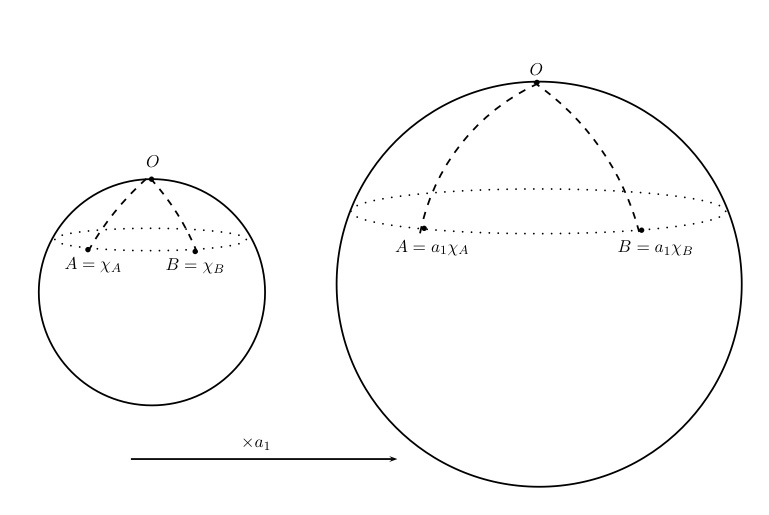
\includegraphics[scale=0.8]{Draw/expansion.png}
\label{}
\end{center}
\caption{A universe-balloon that inflates, growing its size by a factor $a_1$}
\label{expansion}
\end{figure}
Consider the example in Figure \ref{expansion}: if we choose a spherical coordinate system $(\chi,\theta,\phi)$ centered in $O$ ($\chi=0$ corresponds to $O$), we choose two points at distances $\chi_A$ and $\chi_B$ from $O$: if now we inflate the balloon, and its size grows by a factor $a_1$, then all the distances measured on the balloon will grow by the same amount. That is to say, on the inflated balloon, the points $A$ and $B$ will find themselves at a physical distance $a_1\chi_A$ and $a_1\chi_B$ from $O$; nevertheless, we can still identify the points $A$ and $B$ on the inflated balloon, by their \textit{comoving distances} $\chi_A$ and $\chi_B$, provided that we know the \textit{scale factor} $a_1$, that allows us to compute the \textit{physical distances} $\chi_{phys}=a_1\chi$. We will picture our expanding universe in an exacly analogous way: we choose $O$ as our observation point, Earth, and we choose a spherical coordinate system $(\chi,\theta,\phi)$ centered on us (this choice is arbitrary, but 
there's nothing special in it, as the cosmological principle dictates, it is only a matter of convenience): we intend the coordinate $\chi$ as a radial comoving distance, which can be converted into a physical radial distance, if we know the scale factor $a$ of the universe. The statement that the universe expands, means that the scale factor $a(t)$ depends on time, and grows, meaning that physical distances between objects grow as well ($\chi_{phys}=a(t)\chi$); this description gives us a good definition of observers \textit{at rest}: an observer is at rest with the expansion of the universe if its comiving coordinate $\chi$ doesn't change with time. Note that, even if two galaxies are at rest (their comoving distance is the same), their physical distance grows indeed, because it gets multiplied by $a(t)$. This means that the geometry of our homogeneous, expanding universe will be encoded in a metric in the form 
\begin{equation}
\label{frw}
ds^2=-c^2dt^2+a^2(t)\left[d\chi^2+s^2_k(\chi)(d\theta^2 + \sin^2{\theta}d\phi^2)\right]
\end{equation}  
or 
\begin{equation}
g_{\mu\nu}[k,a(t)]=
\begin{pmatrix}
-c^2 & 0 & 0 & 0 \\
0 & a^2(t) & 0 & 0 \\
0 & 0 & a^2(t)s_k^2(\chi) & 0 \\
0 & 0 & 0 & a^2(t)s_k^2(\chi)\sin^2{\theta}
\end{pmatrix}
\end{equation}
This form of the metric is called \textit{Friedmann-Roberson-Walker} metric, from the name of the physicists who first proposed it: this is the most general metric we can write down for an expanding, homogeneous universe. Once we specify the matter content of the universe, encoded in the stress energy tensor $T_{\mu\nu}$, we can plug the metric in the Einstein equation
\begin{equation}
\label{einfried}
G_{\mu\nu}[k,a(t)]=\frac{8\pi G}{c^4}T_{\mu\nu}
\end{equation}
which will translate in a differential equation for $k$ and $a(t)$; we can solve this equation and find the time dependence of the scale factor $a(t)$ to see how fast the universe expands in various scenarios (remember that in this differential equation, which by the way is called \textit{Friedmann equation}, will also make appearence $R$, our comoving curvature scale); before going into these details, however, let's examine some of the important features of a metric in the form (\ref{frw})
\subsection{Cosmological redshift}
What we will try to do in this section, is convince ourselves that a metric in the form \textit{Friedmann-Robertson-Walker} naturally explains the redshift of galaxies that we see in our observations: you already encountered this concept in the previous lecture, interpreting it as a dopplershift; here we will interpret this effect under a slightly different perspective. Consider a light source (for example a galaxy) at a comoving distance $\chi_E$ from us, as in Figure \ref{redshift}
\begin{figure}
\begin{center}
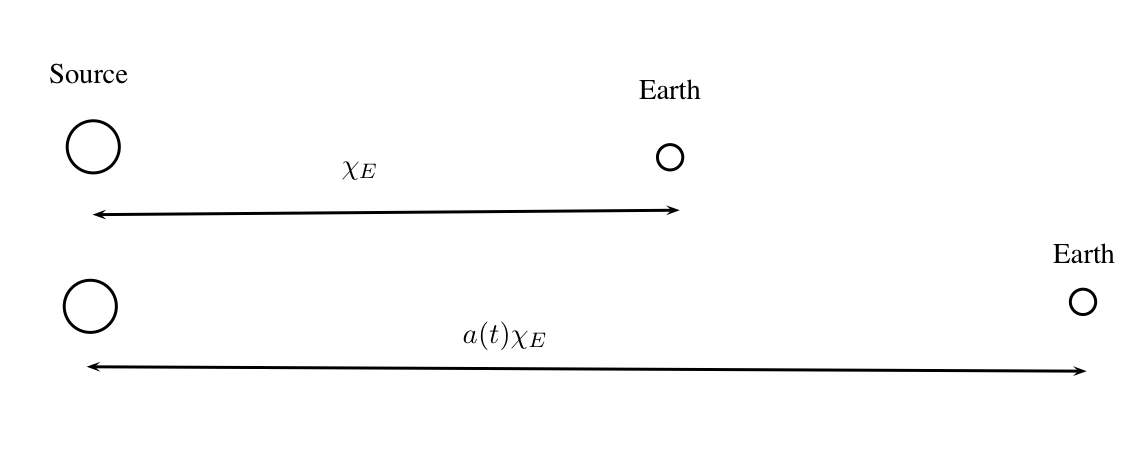
\includegraphics[scale=0.8]{Draw/redshift.png}
\label{}
\end{center}
\caption{A picture explaining cosmological redshift}
\label{redshift}
\end{figure}
This galaxy will emit light at a frequency $f_S$; if both we and the galaxy are at rest with the expansion, the comoving distance between us $\chi_E$ will remain constant, but nevertheless the galaxy will recede from us because the physical distance will grow as $a(t)\chi_E$: this will have the consequence that the light that we receive on earth will have a lower frequency $f_E$.  Now, remember emember that light travels always along null geodesics ($ds^2=0$), so if we have to follow the path of a photon $\chi(t)$ from the galaxy ($\chi=\chi_E$) to us ($\chi=0$), this path must satisfy $ds^2=0$ or $a(t)d\chi=-cdt$. Suppose a photon is emitted from the galaxy at time $t_S$ and is received at earth at a subsequent time $t_E=t_E(t_S)$. It is then true that 
\begin{equation}
\label{comdis}
\chi_E=\int_E^Sd\chi=c\int_{t_S}^{t_E(t_S)}\frac{dt}{a(t)}
\end{equation}
Since the number of photons emitted should be the same of the number of photons receive on earth, it must be true that $f_Edt_E=f_Sdt_S$, which will immediately tell us that if we define a \textit{redshift parameter} associated with our galaxy (that quantifies the difference between emitted and received light frequency) in the obvious way
\begin{equation}
z\equiv \frac{f_S-f_E}{f_E}
\end{equation}
then the following relation must hold
\begin{equation}
z=\frac{dt_E}{dt_S}-1
\end{equation}
Now take equation (\ref{comdis}), differentiate it with respect to $t_S$ taking into account that the comoving distance is constant $\frac{d\chi_E}{dt_S}=0$ to get $\frac{dt_E}{dt_S}=\frac{a(t_E)}{a(t_S)}$. If we call $z_S$ the redshift parameter of our galaxy, which is the quantity that we measure in observations (looking at the shift in the galaxy emission spectra), we immediately get
\begin{equation}
1+z_S=\frac{a(t_E)}{a(t_S)}
\end{equation}
This tells us a fact of the uttermost importance: if by convention we set the scale factor today (at $t_E$) as unity ($a(t_E)=1$), then we see that $a(t_S)=\frac{1}{1+z_S}$, that is to say the redshift of our galaxy is a measure of the scale factor of the universe at the time when the light was emitted. If we knew the time dependence $a(t)$ (for which we have to solve Einstein's equation), then redshift $z$ would provide us with a direct measure of the age of the universe $t(z)$ at which the light that we see was emitted
\subsection{Redshift as a measure of distance}
It happens that, one we exploit at full the properties of the metric (\ref{frw}), we discover that redshift is not only a measure of time, but also of the physical distance $d_E$ between us and the galaxy of which we measure the redshift. We have that
\begin{equation}
d_S=a(t_E)\chi_E=a(t_E)\int_{t_S}^{t_E}\frac{cdt}{a(t)}=\int_{z_S}^0\frac{c}{a(z)}\frac{dt}{dz}dz
\end{equation}
Now take into account that $\frac{dz}{dt}=-\frac{\dot{a}(t)}{a^2(t)}a(t_E)$, and define the \textit{Hubble parameter} as 
\begin{equation}
H(t)=\frac{\dot{a}(t)}{a(t)}
\end{equation}
to get
\begin{equation}
\label{distanceredshift}
d_E(z_S)=\int_0^{z_S}\frac{c}{H(z)}dz
\end{equation}
Note that the Hubble parameter $H(t)$ has units 1/time, and is a measure of the expansion rate of the universe; moreover, it is completely insensible to the convention we used $a(t_E)=1$. Its value today $H(t_E)=H_0$ is called \textit{Hubble constant}, and is measured to be $H_0=100h\,\mathrm{km}\,\mathrm{s}^{-1}\mathrm{Mpc}^{-1}$ with $h\sim 0.7$. Note also that, in order to convert redshift $z$ in a measure of time and distance, we first need to solve the Friedmann equation to get the dependency $a(t)$, which in the end depend on the matter content of our universe. We will get to this in the next section. 

\section{The Friedmann equation}
What we want to do in this section is mainly find a way to compute the evolution of the scale factor $a(t)$; as pointed out in the previous paragraphs, in order to do that we need to know the matter content of the universe (what is it made of) and then solve Einstein's equation (\ref{einfried}) for $a$. Before going into this, though, we need to see how this equation looks like when we write it down in terms of $a$ and $\dot{a}$.
\subsection{The matter content of the universe}
As we pointed out before, we model our universe, at a first approximation, as a uniform inflating ball filled of some homogeneous fluid of density $\rho$: in the previous section we focused on what are the physical and observational consequences of this expansion, now we want to focus on \textit{the meachanism} that triggers this size growth. It turns out that, according to general relativity, what causes the expansion is the universe itself, or better, the matter it is made of. This homogeneous fluid that permeates our balloon might have different components that have different characteristics and have different physical consequences. We describe these different components in term of their energy momentum tensor $T_{\mu}^{\nu}$; we distiguish two main contributions to the overall energy budget:
\begin{itemize}
\item Ordinary matter and dark matter: these kind of components are described by perfect fluids of uniform density $\rho$ and pressure $P$, which are connected by the so called \textit{equation of state} $P=w\rho c^2$. The number $w$ specifies the type of matter we are considering; over 75\% of the overall matter budget in our universe is made by \textit{dark matter}, which does not interact with light and hence cannot be seen directly in observations, and today is only indirectly detected observing its gravitational effects. The true nature of dark matter is still unknown (we will get to this towards the end of the course). All this matter content is described by an energy momentum tensor in the form 
\begin{equation}
T_{\mu,M}^\nu=(P+\rho c^2)U_\mu U^\nu + P\delta_\mu ^ \nu
\end{equation} 
Where $U^\mu$ is the 4-velocity of the fluid elements (in units of $c$) and, if this fluid is homogeneous and at rest with the expansion, then this 4-velocity is forced to have the form $U^\mu=\left(\frac{dt}{dt},\frac{d\chi}{dt},\frac{d\theta}{dt},\frac{d\phi}{dt}\right)=(1,0,0,0)$
\item Dark energy: the presence of this component in the overall energy budget is probably one of the most tricky unsolved mysteries in science. Nevertheless its presence is required by current observation of the accelerated expansion of the universe; its energy momentum tensor can be written in the form
\begin{equation}
T_{\mu,DE}^\nu=-\frac{\Lambda c^4}{8\pi G}\delta_\mu^\nu
\end{equation}
With $\Lambda$ a suitable constant with units length$^{-2}$; why immediately see why this kind of energy source is really particular. It can be indeed thought as some kind of fluid with equation of state $P=-\rho c^2$, i.e. a fluid with \textit{negative} pressure: if ordinary and dark matter exert a positive pressure telling the universe to stop expanding (exerting positive gravity), this kind of dark energy tells us exacly the opposite, it exerts a negative gravity that pushes out and accelerates the expansion of the universe! Moreover, current observations of the CMB and galaxy surveys tell us that not only this weird dark energy is there, but it makes up for more that 70\% of the overall energy budget. The natural question we may ask then is: where does it come from? And the answer is again ''we don't know''; current observations today measure $\Lambda \approx 10^{-52}\mathrm{m}^{-2}$, which translates in a physical length scale of $1/\sqrt{\Lambda}\approx 10^{26}\mathrm{m}\approx 3\mathrm{Gpc}$. Beside 
the pure coincidence fact that this length scale equals the size of the observable universe today, this length scale is extremely mysterious: there is no current physical theory, neither general relativity nor the standard model in which this length scale emerges naturally. The origin of this \textit{cosmological constant} $\Lambda$ is hence still unknown. 
\end{itemize}
\subsection{The evolution equation} 
If we plug in $T_{\mu,M}^\nu$ and $T_{\mu,DE}^\nu$ in the right hand side of (\ref{einfried}) and work out the proper differential calculations, we end up with a differential equation for $a(t)$, that takes the remarkable form 
\begin{equation}
\label{friedmanneq}
\left(\frac{\dot{a}(t)}{a(t)}\right)^2=\frac{8\pi G}{3}\rho[a(t)]-\frac{kc^2}{R^2a^2(t)}+\frac{\Lambda c^2}{3}
\end{equation}
This is a proper differential equation for $a(t)$ that takes the name of \textit{Friedmann equation} and, as promised, ties together the energy properties ($\rho$ and $\Lambda$) and the geometrical properties (the scale factor $a$ and the curvature scale $Ra$) on our physical system. This equation can in principle be solved to get the explicit dependence of $a$ in terms of $t$, except that we still don't know how the fluids' densities depend on the size of the universe $a$. This will be our next goal
\subsection{A little bit of thermodynamics}
To understand how the densities of the various matter components scale with $a$ we have to apply nothing more than the first principle of thermodynamics, which says that the change of energy $dE$ of a physical system is given by the heat that flows in $dQ$ minus the work done by the system $dW=PdV$, being $V$ and $P$ the volume and pressure of the system: $dE=dQ-PdV$. Since in our case the universe is an isolated system, there is no heat flowing in nor flowing out $dQ=0$ and we can use $E=\rho a^3$ and $V=a^3$ to get
\begin{equation}
d(\rho a^3)=-Pd(a^3)=-w\rho d(a^3)
\end{equation}
For a component with equation of state $w$; working out the calculations, this equation can be simplified into 
\begin{equation}
\frac{d\rho}{\rho}=-3(1+w)\frac{da}{a}
\end{equation}
Which in the end leads to a scaling 
\begin{equation}
\rho(a)=\rho(a_0)\left(\frac{a}{a_0}\right)^{-3(1+w)}
\end{equation}
It turns out that the total matter budget of the universe can be divided into two main classes:
\begin{itemize}
\item ''Cold'', non relativistic matter, made of particles which move with speeds $v\ll c$; today, all ordinary matter (electrons, protons, nuclei, atoms) as well as dark matter belong to this category. For this kind of matter, one can estimate the equation of state index as 
\begin{equation}
w=\frac{P}{\rho c^2}=\frac{k_B T}{mc^2}\approx \left(\frac{v}{c}\right)^2\ll 1
\end{equation}
Where $T$ and $m$ are respectively the temperature and particle mass associated with this particular component: for the sake of this lecture we can safely set $w=0$ for this ''cold'' matter and obtain a scaling $\rho_c(a)\propto a^{-3}\propto (1+z)^3$
\item ''Hot'', relativistic matter, made of particles which move with speeds close to the speed of light $v\sim c $ : both photons (massless) and neutrinos (which have very little mass) belong to this category. Relaticistic thermodynamics tells us that this "hot" matter can be described in terms of an equation of state index of $w=1/3$ and hence the density for these particular fluid components should scale as $\rho_h(a)\propto a^{-4}\propto (1+z)^4$
\end{itemize}
\subsection{Some particular solutions to the Friedmann equation: how to measure the age of the universe}
We have seen in the previous section that some of the components our universe is made of exibit a simple scaling in their density $\rho(a)\propto a^{n}$. Suppose we wish to solve the Friedmann equation (\ref{friedmanneq}) assuming our universe is flat ($k=0$ or $R=\infty$), contains no dark energy ($\Lambda = 0$, this is unrealistic but helps us make some estimates) and contains only one fluid component described by an equation of state index $w$ (which in real cases can be 0 or 1/3). Then our Friedmann equation will simplify enormously and reduce to 
\begin{equation}
\left(\frac{\dot{a}(t)}{a(t)}\right)^2=\frac{8\pi G\rho_0}{3a_0^n}[a(t)]^n
\end{equation}
Since the choice of $a_0$ is arbitrary, this equation has no natural timescale built in, and hence we seek a solution in the form $a(t)=Ct^\lambda$, with $C$ and $\lambda$ some constant numbers. We have little interest in the normalization constant $C$, since it can always be set to 1 redefining the scale factor at some particular time (as we did with our convention $a(t_E)=1$), what we are really interested in is the exponent $\lambda$, which is the one that tells us how fast the universe expands. Matching the powers of $t$ on the left and right hand side of the equation above gives us the relation $-2=\lambda n$ and hence $\lambda=-2/n$, and an overall solution
\begin{equation}
a(t)=a(t_E)\left(\frac{t}{t_E}\right)^{\frac{2}{3(1+w)}}
\end{equation}
Which gives us the dependencies $a(t)\propto t^{2/3}$ if only cold matter is present and $a(t)\propto t^{1/2}$ if only hot matter is present. Moreover, we can express the Hubble constant today as
\begin{equation}
H_0=\frac{\dot{a}(t_E)}{a(t_E)}=\frac{2}{3(1+w)}\frac{1}{t_E}
\end{equation}
If we think about it a little bit, this last equation gives us an expression for the age of the universe today, which is nothing more than $t_E=2/[3(1+w)H_0]$: both in the cold case $w=0$ and in the hot case $w=1/3$ this relation gives us an estimate for the age of the universe $t_E\approx 10$\,Gyr, which is not that far from the number you get if you were to consider the full matter + dark energy + curvature model. 
Let's consider another naive but interesting example: if our universe were to be flat and contain no matter at all, but just dark energy, the friedmann equation would reduce to
\begin{equation}
\frac{\dot{a}(t)}{a(t)}=\sqrt{\frac{\Lambda c^2}{3}}\equiv H_0
\end{equation}
which would have a solution $a(t)=a(t_E)e^{H_0(t-t_E)}$, i.e. would describe an exponential, \textit{accelerated} expansion with $\ddot{a}(t)>0$; compare this to the previous studied case with matter only: you may convince yourselves that these matter only models describe a \textit{decelerated} expansion with $\ddot{a}(t)<0$. That's what dark energy does for us: it pushes out and accelerates our universe's expansion, helping us explain the experimental data we see (which strongly indicate an accelerated expansion). When we consider a more realistic model, a flat universe with both dark matter and dark energy (the so called $\Lambda$CDM model, in which matter makes up for 1/4 and dark energy for 3/4 of the overall energy budget, as observations suggest) we get a more complicated time dependence 
\begin{equation}
\frac{a(t)}{a(t_E)}=\left[\frac{\sinh{\left(\frac{3\sqrt{\Omega_\Lambda}H_0 t}{2}\right)}}{\sinh{\left(\frac{3\sqrt{\Omega_\Lambda}H_0 t_E}{2}\right)}}\right]^{2/3}
\end{equation}
With $\Omega_\Lambda=\frac{\Lambda c^2}{3H_0^2}\approx 0.75$; we'll talk more about this model in the following chapter. For the moment, you can lookup at table \ref{timez} that outlines some of the most important events in the universe's history, with the time-redshift conversion made according to the flat $\Lambda$CDM model

\begin{table}[htbp]
\begin{center}
\begin{tabular}{|c|c|c|} \hline
\textbf{Event} & \textbf{Redshift}$z$ & \textbf{Corresponding time}($\Lambda$CDM) \\ \hline
Big bang & $\infty$ & 0 \\ \hline
Cold and hot matter density is the same & 3200 & $6\cdot 10^4$yr \\ \hline
Decoupling, origin of the CMB & $10^3$ & $3\cdot 10^5$yr \\ \hline
Reionization & $10$ & $0.5$Gyr \\ \hline
Today& 0 & $13$Gyr \\ \hline
\end{tabular}
\end{center}
\caption{Some important event's in the universe's history}
\label{timez}
\end{table}